\documentclass[tikz,border=2pt]{standalone}
\usepackage{pgfplots}
\pgfplotsset{compat=1.18}
\usetikzlibrary{intersections}
\usepgfplotslibrary{fillbetween}


\begin{document}
	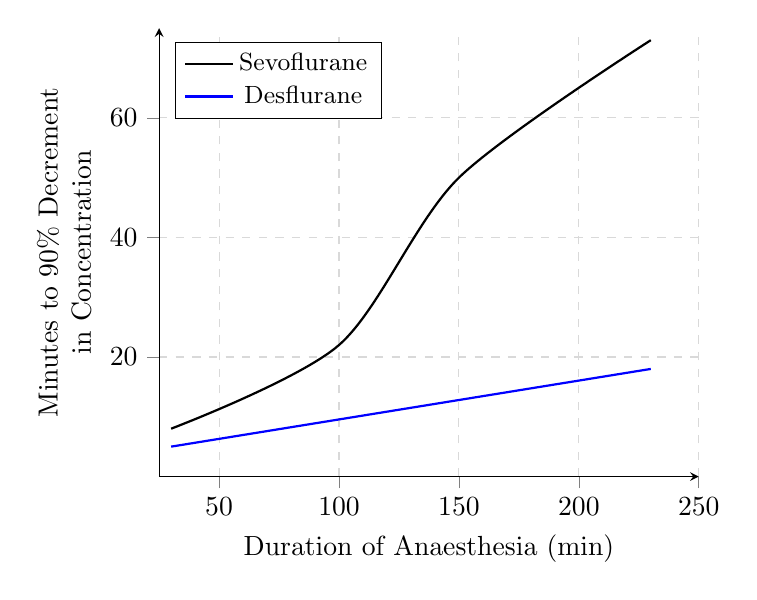
\begin{tikzpicture}
		\begin{axis}[
			axis lines=middle,
			ymin = 0,
			ymax = 75,
			xmin = 25,
			xmax= 250,
			grid = major,
			grid style={dashed, gray!30},
			ylabel near ticks,
			xlabel near ticks,
			xlabel= Duration of Anaesthesia (min),
			ylabel= Minutes to 90\% Decrement \\ in Concentration,
			ylabel style ={align=center, text width=5cm},
			tick align=outside,
			legend pos= north west,
			legend style={font=\small, cells={align=left}}]

			\draw[black, thick] plot[smooth,tension=0.5] coordinates {(axis cs: 30,8) (axis cs: 100,22) (axis cs: 150, 50)  (axis cs: 230,73)};
			\draw [blue, thick] (30,5) -- (230,18);

			\addlegendimage{black, thick}
			\addlegendentry{Sevoflurane}
			\addlegendimage{blue, thick}
			\addlegendentry{Desflurane}

		\end{axis}
	\end{tikzpicture} 
\end{document}